\chapter{About the technology stack}
\label{cha:techstack}

Before describing the entire project, we need to know what we are talking about. In particular, there are the softwares or libraries strongly used in the project:  
\begin{itemize}
    \item Docker
    \item ROS2
    \item Gazebo
    \item Navigation stack, nav2
    \end{itemize}

\section{Docker}

% insert introduction
Docker was used (impiegato?) because of two reasons:
\begin{itemize}
    \item permit (?) development on any computer not running necessarily Ubuntu 20.04 (?) as its OS
    \item keep the workspace equal for every device
    \item separate current workspace from all the other ones, to avoid conflicts or dependencies problems
\end{itemize}  

Since there are multiple people working on this robot with their own projects, it is a bad practice to mix everything together. % continue

Indeed, the entire project comes with a Dockerfile with the needed setup and packages required to develop and run the real robot or the simulation; if someone wants, (?) could still install everything by hand\footnote{See attachment for the dependencies required or Dockerfile attachment} on its own system.


\section{\acrshort{ros}2}

% https://www.allaboutcircuits.com/technical-articles/an-introduction-to-robot-operating-system-ros/#:~:text=ROS%20is%20designed%20to%20be,using%20the%20publish%2Fsubscribe%20model., 04/08
% https://docs.ros.org/en/foxy/index.html, 27/07

{\it \acrshort{ros}2, which stands for Robot Operative System 2, is a set of software libraries and tools for building robot applications.}\cite{ros2desc} On it, every process is a node and each node has the possibility to talk to other ones thanks to some channel of communications called topics. How? Using the publish/subscribe model.

ROS is an OS in concept because it provides all the services that any other OS does—like hardware abstraction, low-level device control, implementation of commonly-used functionality, message-passing between processes, and package management.\footnote{allaboutcircuits.com, 04/08}

In other words, executing a ROS node on your computer is the same of executing it on a robot, as long as you are using the same external devices. Or maybe, you don't need to.

\section{Gazebo}

Here comes the simulation part, because thanks to Gazebo-ROS integration it is possible, with some additional libraries, to simulate external devices. It is not limited to this, because it gives you a sandbox you could set up as the real environment you want to simulate.

In this way, you don't need to have the real robot next to you, you can just use a virtual one: it's very useful in the case you want to change some algorithms or parameters, and you need to test them even if you are on the opposite side of the world.

% includere il fatto che l'ho fatto per questo motivo la parte di simulazione?

\section{rviz2}

Rviz2, is a visualization tool for ROS: in this way, you are able to visualize the sensors, the robots, the environment, and also the algorithms; in general, you can see the actual state of your \acrshort{ros} system.

\section{\acrfull{nav2}}

The Navigation Stack is a collection of packages of \acrshort{ros}2 which provides useful tools helping you with the navigation of your robot: path planning, localization, and so on. You can use it by passing your desired configurations in a YAML file which will be used when you launch the navigation stack: basically, you specify what nodes you want to use and the parameters you want to set, and everything is done for you. (?)
These packages were used as a base to everything else, so in this way I don't need to worry about the navigation algorithms, since my goal is to develop a system to move around ground robots where indicated.

\begin{figure}[h]
    % \noindent\makebox[0.9\textwidth]{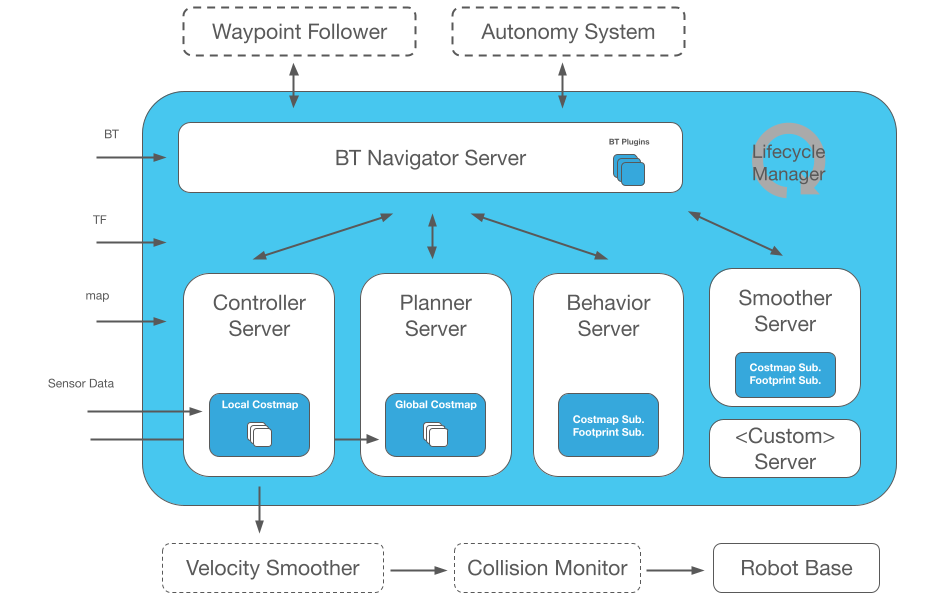
\includegraphics[width=0.9\paperwidth]{images/nav2_architecture}}
    \centering
    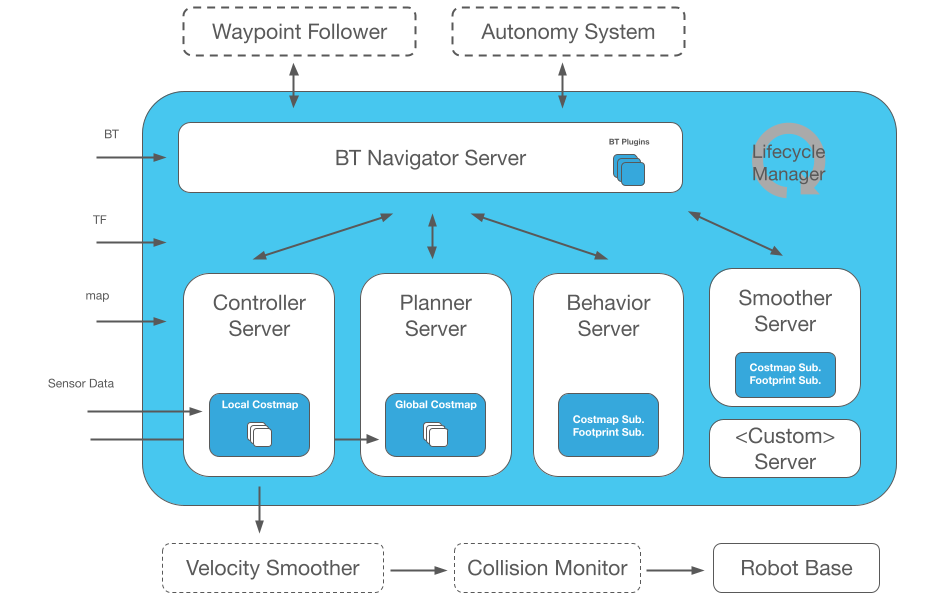
\includegraphics[width=0.8\textwidth]{images/nav2_architecture}
    \caption{Navigation architecture}
  
  \end{figure}
